\chapter{Implementation - Motion Planning}

This chapter will cover the implementation methods on motion planning side of this project. The entire code for this part can be seen in !!!!!!!!!!

\section{MoveIt! Interface and Planning Scene Setup}
As mentioned in Background Chapter, the motion planning part will utilize MoveIt!. The $moveit\_commander$ namespace is imported in order to use Python MoveIt! interface. This namespace contains a $RobotCommander$ class, a $MoveGroupCommander$ class, and a $PlanningSceneInterface$ class.

A $RobotCommander$ object is firstly instantiated called $robot$. This object is the outer-level interface to the robot, which allow user to catch YuMi's names of joints, groups, and links and easy access to their properties.

To plan and execute motions on the YuMi, $MoveGroupCommander$ objects need to be instantiated as well. Each object should be one group of joints. In this case, the group can be $left\_arm$, $right\_arm$, and $both\_arms$. All of them are defined with the following settings.

\begin{table}[H]
\centering
\resizebox{\columnwidth}{!}{
\begin{tabular}{||c|c|c|c||}
\hline
Pose reference frame & Allow re-planning & Goal position tolerance & Goal orientation tolerance \\ \hline\hline
$yumi\_body$ & False & 0.005 & 0.005 \\ \hline
\end{tabular}}
\caption{Settings of three $MoveGroupCommander$ objects}
\label{armsetup}
\end{table}

Moreover, a $PlanningSceneInterface$ object is instantiated, which is an interface to the world surrounding the robot. In this case, I defined the 3D position and 3D dimension of the workbench in front of YuMi. By doing this, the workbench will be regarded as an obstacle to YuMi, so that the potential collisions between YuMi's arm(s) and the workbench can be avoided. However, the external cameras are not defined due to high measurement difficulty, by setting some safe positions for YuMi, the collisions can also be avoided. The details are discussed in Section \ref{safetyposescalculation}.

\begin{figure}[H]
\centering

\includegraphics[width = 0.5\columnwidth]{images/ph.png}
\caption{The planning scene}
\label{scene}
\end{figure}

Finally, a $DisplayTrajectory$ publisher is created, which is utilized to publish trajectories for RViz to visualize:

\begin{minted}[frame=single, framesep=1.5mm, baselinestretch=1, fontsize=\footnotesize, linenos, breaklines]{python}
display_trajectory_publisher = rospy.Publisher('/move_group/display_planned_path', 	moveit_msgs.msg.DisplayTrajectory, queue_size=20)
\end{minted}


\section{Movement Control}
The opening and closing of YuMi' gripper(s) depend on the gripper effort value, which needs to be set between $-20$ to $20$. The gripper will open when the value is negative and close when it is positive. By publishing the effort value of specific gripper to its corresponding topic, $/yumi/gripper\_r\_effort\_cmd$ for right gripper, or $/yumi/gripper\_l\_effort\_cmd$ for left gripper, the gripper control function can be achieved. (Whether the command is to open or close, the effort value will eventually set to 0 in order to relax the effort, which will not change the gripper state.)

As for YuMi's arm(s) control, it can be implemented in two ways: setting a joint goal or setting a pose goal.

\begin{itemize}
    \item \textbf{Joint Goal:} Each of YuMi's arm has 7 joints (shown in Figure \ref{yumijoint}). By setting them to specific value, every joint on the arm will rotate or bend accordingly to that configuration. The position of end-effector can be computed using forward kinematics.
    
    In this project, this approach is only used to adjust YuMi's arm(s) to safe positions through the manipulation process, which will be introduced in Section \ref{safetyposescalculation}.
\end{itemize}

\begin{figure}[H]
\centering
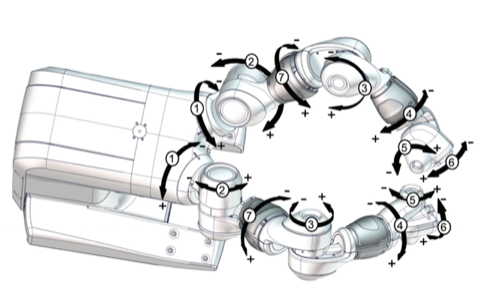
\includegraphics[width = 0.7\columnwidth]{Implementation/mp/yumijoints.png}
\caption{Joints of YuMi's arms \citep{Productspecification}}
\label{yumijoint}
\end{figure}

\begin{itemize}
    \item \textbf{Pose Goal:} The movement of a group can also be controlled by setting a pose goal for YuMi's end-effector(s) directly. The pose contains 3D position (x, y, z) and 3D orientation information (roll, pitch, yaw). The joint parameters that achieve this pose can be calculated via inverse kinematics. Notice that for the same pose goal, the joint parameters can be different.
    
    This method is used throughout the manipulation process including adjusting shoe pose, putting the lace through shoe hole, and grabbing the shoelace etc.
\end{itemize}

For single arm manipulation, letting the end-effector move to a pose goal can be achieved in two ways. Either using $compute\_cartesian\_path$ or $set\_pose\_target$ function. For a given pose goal, the former method will be tried first, and if it fails, the later one will be used. The $compute\_cartesian\_path$ function computes a Cartesian path that follows specified waypoints (6D poses). The maximum resulting step size between the end-effector configurations of consecutive points in the result trajectory is predefined, which is 0.01 and provides a resolution of $1$ cm. Collision and kinematic will be checked and if these constraints cannot be met, the function will return a fraction of the path achieved between $0$ and $1$. If successful, fraction will equal to $1$.

\begin{minted}[frame=single, framesep=1.5mm, baselinestretch=1, fontsize=\footnotesize, linenos, breaklines]{python}
(plan, fraction) = cur_arm.compute_cartesian_path(waypoints, 0.01, 0.0, True)
\end{minted}

While the $set\_pose\_target$ function can be used for both single and dual arm motion planning. Its inputs are simply the target 6D pose and the name of corresponding end-effector. Following is the dual arm plan and move function for this project utilizing $set\_pose\_target$. 

\begin{minted}[frame=single, framesep=1.5mm, baselinestretch=1, fontsize=\footnotesize, linenos, breaklines]{python}
def plan_and_move_dual(target_l, target_r):
    group_both.set_pose_target(target_l, "yumi_link_7_l")
    group_both.set_pose_target(target_r, "yumi_link_7_r")
    plan = group_both.plan()
    group_both.go(wait=True)
    rospy.sleep(3)
\end{minted}



\section{Safe Positions Calculation} \label{safetyposescalculation}

\begin{figure}[H]
\centering
\subfigure[cal]{
\includegraphics[width = 0.32\columnwidth]{images/ph.png}}
\subfigure[home]{
\includegraphics[width = 0.32\columnwidth]{images/ph.png}}
\subfigure[initial]{
\includegraphics[width = 0.32\columnwidth]{images/ph.png}}
\caption{Safe positions of YuMi}
\label{safeposition}
\end{figure}

Figure \ref{safeposition} shows three pre-defined safe positions of YuMi: cal position, home position and initial position. For each manipulation, YuMi will start with cal position, then move to either home or initial position before perform the tasks. Once it finishes the job, it will move back to home or initial position before finally returning to cal position. By doing so, YuMi's arm(s) will always moving in front of and under the cameras, which prevents potential collisions between them.

After moving YuMi's arm(s) to these desired positions in Rviz, the joint parameters ($safeJointPositionR$ and $safeJointPositionL$) are measured by using $get\_current\_joint\_values$ function. For each safe position, the joint goal(s) can the be set accordingly. Following is the code example to plan and move both arms to a safe position.

\begin{minted}[frame=single, framesep=1.5mm, baselinestretch=1, fontsize=\footnotesize, linenos, breaklines]{python}
elif (arm == BOTH):
    group_both.set_joint_value_target(safeJointPositionL + safeJointPositionR)
    group_both.plan()
    group_both.go(wait=True)
\end{minted}

\section{Shoe Pose Adjustment} \label{adj}

\begin{figure}[H]
\centering

\includegraphics[width = 0.5\columnwidth]{images/ph.png}
\caption{Shoe pose adjustment 2d ppt flow chart!!!}
\label{adjust}
\end{figure}

As mentioned in Section \ref{shoedetection}, if the shoe is vertically placed, then its orientation needs to be adjusted. The idea is illustrated in Figure \ref{adjust}, in which YuMi will use both arms. These waypoints in the adjustment process are computed using the same approach as the shoe hole (Section \ref{3dlocationestimation}), by converting the 2D pixel positions around the shoe ($adr$, $adrr$, $adl$, $adll$) to the real-world coordinates, then utilizing $TF$ to obtain the location referenced to $yumi\_body$ frame using $lookupTransform$ function. Following is the example applied on location $adr$.

\begin{minted}[frame=single, framesep=1.5mm, baselinestretch=1, fontsize=\footnotesize, linenos, breaklines]{python}
(trans_adr,_) = self._tfsub.lookupTransform('/yumi_body', '/adr', rospy.Time(0))
\end{minted}

The output $trans\_adr$ is the 3D location I want, !!!!! the pose !!!!!1

by firstly moving YuMi end-effectors to these pre-adjustment positions with  !!!!! angle. Then both arms will following the arrows and move towards the middle. After adjustment, they will return to the pre-adjustment positions and move back to cal positions.

\begin{figure}[H]
\centering
\subfigure[]{
\includegraphics[width = 0.19\columnwidth]{images/ph.png}}
\subfigure[]{
\includegraphics[width = 0.19\columnwidth]{images/ph.png}}
\subfigure[]{
\includegraphics[width = 0.19\columnwidth]{images/ph.png}}
\subfigure[]{
\includegraphics[width = 0.19\columnwidth]{images/ph.png}}
\subfigure[]{
\includegraphics[width = 0.19\columnwidth]{images/ph.png}}
\caption{Example of real shoe pose adjustment process}
\end{figure}

Figure \ref{preposeadjust} shows the detected shoe hole before and after adjustment, the later gives a much more accurate results. Figure \ref{shoeposerange} illustrates the ideal orientation range of the shoe hole after adjustment. The hole should face towards the camera, either to its top-left or top-right.

\begin{figure}[H]
\centering
\subfigure[Detected shoe hole before and after adjustment]{
\includegraphics[width = 0.3\columnwidth]{images/ph.png} \label{preposeadjust}}
\subfigure[Ideal orientation range of shoe hole]{
\includegraphics[width = 0.3\columnwidth]{images/ph.png} \label{shoeposerange}}
\caption{}
\end{figure}


\section{Robot Gripper Approaching Pose}
When the orientation of the shoe is ideal, YuMi will start to put the shoe lace into the hole by using the computed $shoe\_hole$ and $pre\_put$ information. Same as the method used in previous section, these two locations are firstly transformed to $yumi\_body$ frame, which gives the coordinates of (xn, yn, zn) and (x, y, z). 

\begin{figure}[H]
\centering
\subfigure[Ideal gripper orientation]{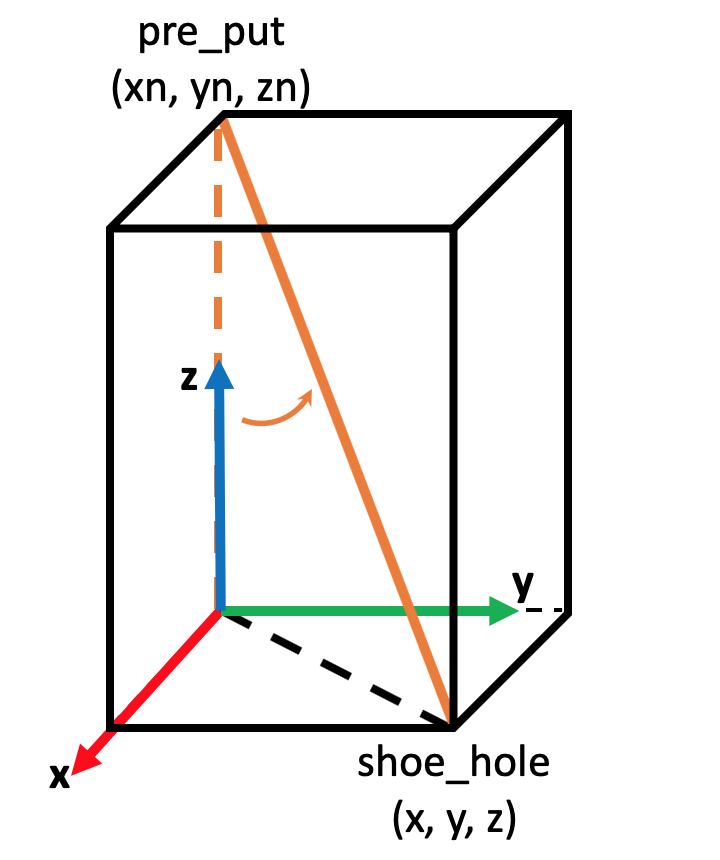
\includegraphics[width = 0.31\columnwidth]{Implementation/mp/ap1.png} \label{gripperap}}
\subfigure[Roll rotation]{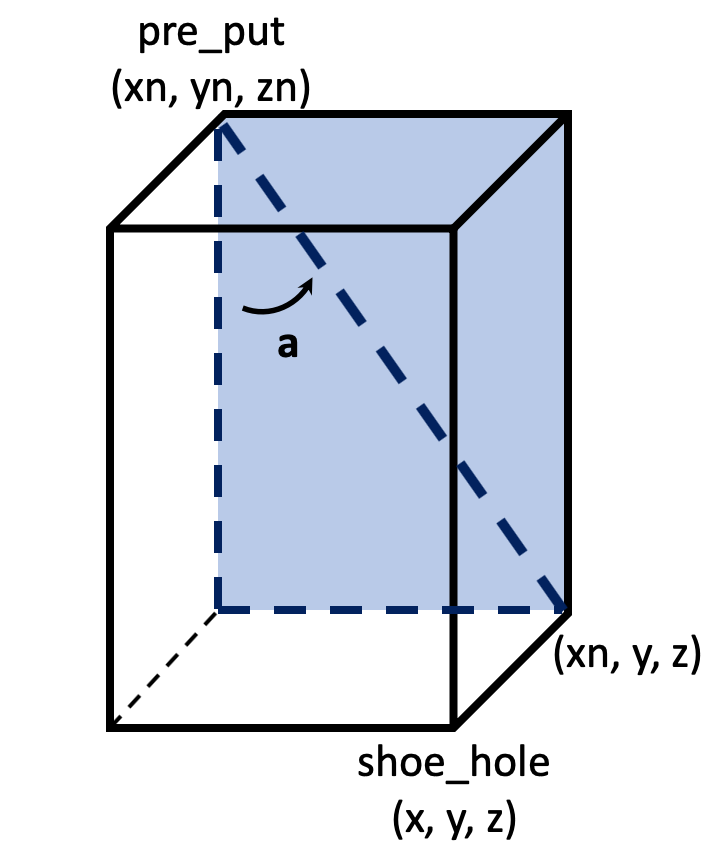
\includegraphics[width = 0.31\columnwidth]{Implementation/mp/ap2.png} \label{roll}}
\subfigure[Pitch rotation]{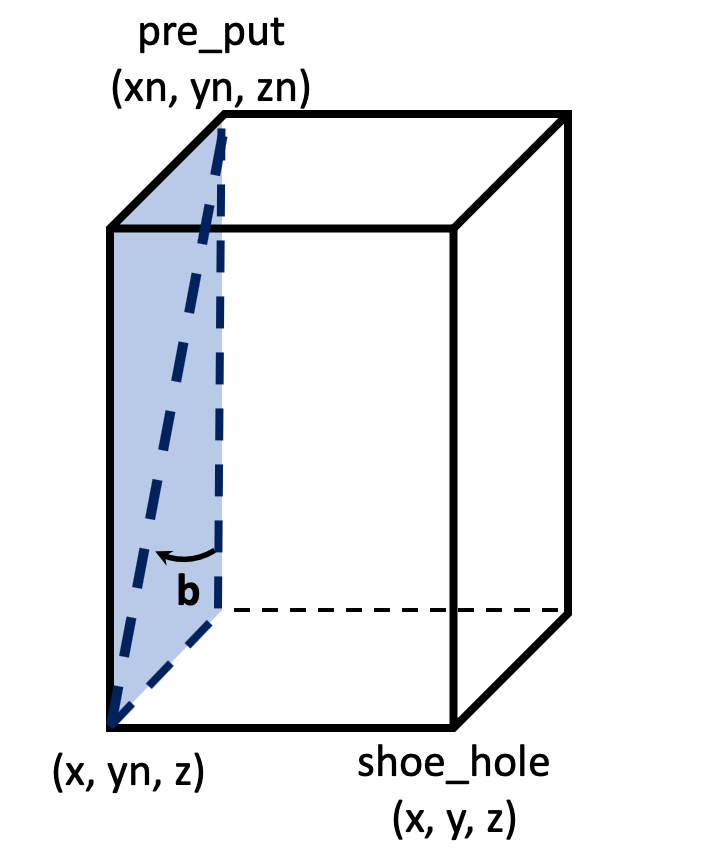
\includegraphics[width = 0.31\columnwidth]{Implementation/mp/ap3.png} \label{pitch}}
\caption{Gripper approaching orientation computation for top-left case}
\end{figure}

Recalling the project requirements, before YuMi starts to manipulate the shoelace, one of its grippers is holding it. In this project, the beginning orientation of the shoelace is considered to be the same as that of the gripper. Therefore, to put it into the shoe hole, the orientation (roll, pitch, yaw) of gripper\slash shoelace needs to be aligned with the normal vector of the plane surrounding with shoe hole. As shown in Figure \ref{gripperap}, for the situation when the shoe hole is orienting to its top-left, this direction is represented as the solid orange line. 

When gripper is facing the ground (the orange dash line in Figure \ref{gripperap}), it has 3D rotation $(0, \pi, \pi)$. Therefore, the alignment can be split into two steps: roll alignment (Figure \ref{roll}) and pitch alignment (Figure \ref{pitch}). There is no need to consider yaw alignment for this step, because the shoelace insertion will not be affected no matter what angle it is. Thus, yaw will be kept as $\pi$.

\begin{equation}
a = \arctan \frac{y - yn}{zn - z}
\label{rollcalculation}
\end{equation}

\begin{equation}
b = \arctan \frac{x - xn}{zn - z}
\label{pitchcalculation}
\end{equation}

By using Equation \ref{rollcalculation} and \ref{pitchcalculation}, the roll and pitch angles can be computed. Because the shoe is assumed in an ideal pose (orienting to its top-left or top-right), $a$ will be in the interval $[-\frac{\pi}{2}, \frac{\pi}{2}]$ and $b$ always lies in range $[0, \frac{\pi}{2}]$. Recall that the beginning configuration of gripper pitch angle is $\pi$, therefore the finally 3D orientation of YuMi gripper should be $(a, b + \pi, \pi)$. 

So far, the preliminary pre-put pose is $[xn, yn, zn, a, b + \pi, \pi]$ and the preliminary insertion pose is $[x, y, z, a, b + \pi, \pi]$. However, these poses are not accurate enough for this precision task, whose offsets need to be further adjusted.

\section{Offset Adjustment}
When letting YuMi's gripper move to a specific 3D location with default orientation $(0, \pi, \pi)$ (facing the ground), the system needs to add $-0.025$ offset on the x-axis ($x\_offset$), $0.005$ offset on the y-axis ($y\_offset$), and $0.145$ offset on the z-axis ($z\_error$) to achieve relatively precise movement. However, the offset adjustment becomes complicate when considering the gripper's orientation.

\begin{figure}[H]
\centering
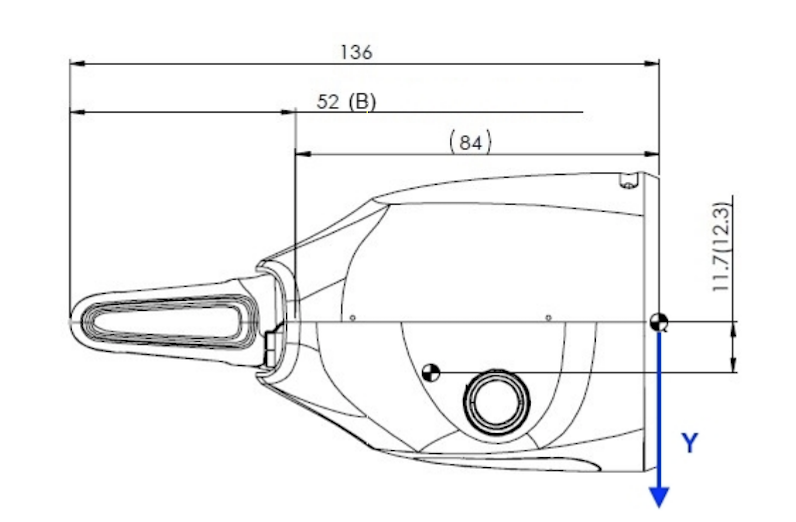
\includegraphics[width = 0.8\columnwidth]{Implementation/mp/gripperoffset.png}
\caption{YuMi's gripper design, adopted from \citep{Productspecification}}
\label{gripperoffset}
\end{figure}

When planning and moving YuMi's arm(s) by setting pose goals, it is all about the pose of the end-effector. Figure \ref{gripperoffset} shows the design of the YuMi' gripper. It can be discovered that the distance between the endpoint of the gripper and the end-effector is $136mm$. Therefore the offset on z-axis contains $0.136$ gripper offset and $0.009$ system offset ($z\_offset$).

\begin{figure}[H]
\centering
\subfigure[X-axis offset due to pitch rotation]{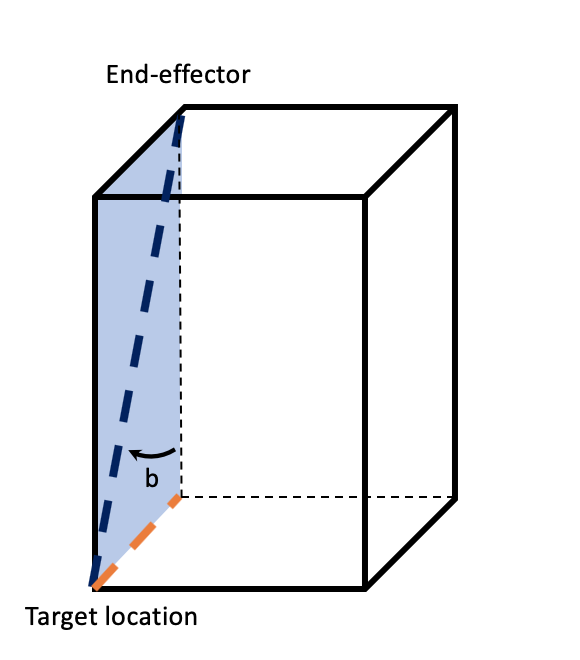
\includegraphics[width = 0.32\columnwidth]{Implementation/mp/off3.png}\label{offsetx}}
\subfigure[Y-axis offset due to roll rotation]{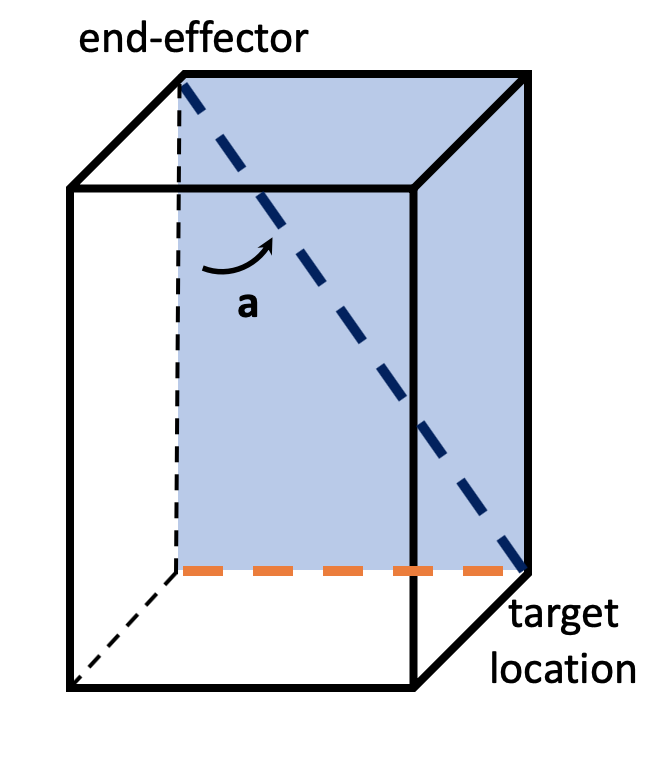
\includegraphics[width = 0.32\columnwidth]{Implementation/mp/off2.png}\label{offsety}}
\subfigure[Z-axis offset due to roll and pitch rotation]{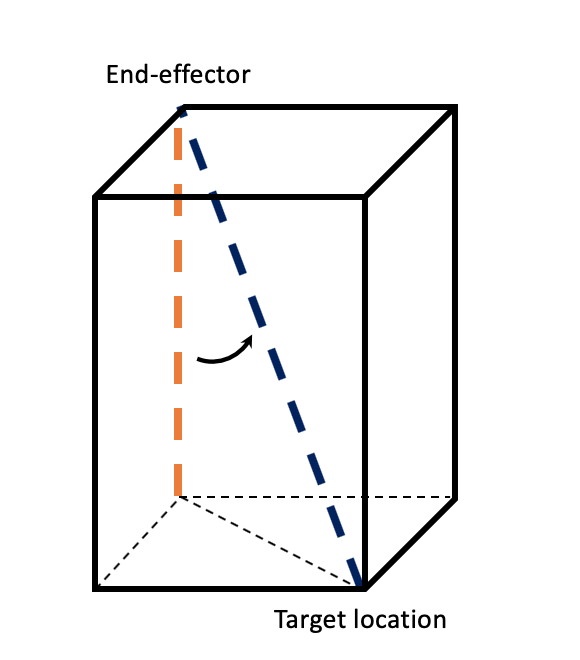
\includegraphics[width = 0.32\columnwidth]{Implementation/mp/off1.png}\label{offsetz}}
\caption{Gripper offset adjustment for top-left case}
\label{offset}
\end{figure}

Once the gripper performs rotations, this gripper offset will affect the (x, y, z) location the gripper endpoint reaches. In Figure \ref{offset}, the dark blue dash lines represent gripper offset, the orange dash lines are the corresponding offsets introduced by it. For Figure \ref{offsetx}, if the gripper has a pitch angle of $b$ and the endpoint of the gripper needs to reach the target location, the end-effector only should be at location "End-effector". The same issue occurs for roll rotation as well (see Figure \ref{offsety}). Furthermore, z-axis offset is affected by both of them. To reach the same target location with rotations, the end-effector needs to move down more than that in default orientation. This is because the influence of gripper offset on the z-axis is diluted by the other two axes.

\begin{equation}
xoff = x\_offset - gripper\_offset*sin(b)
\label{xoff}
\end{equation}

\begin{equation}
yoff = y\_offset - gripper\_offset*sin(a)
\label{yoff}
\end{equation}

\begin{equation}
zoff = gripper\_offset*cos(a)*cos(b) + z\_offset
\label{zoff}
\end{equation}

Equation \ref{xoff}, \ref{yoff}, and \ref{zoff} provide the approach to calculate the final offsets. The final pose goals for putting the shoelace into a hole are illustrated in Equation \ref{Preput} and \ref{Insertion}.

\begin{equation}
Preput\_pose = [xn + xoff, yn + yoff, zn + zoff, a, b + \pi, \pi]
\label{Preput}
\end{equation} 

\begin{equation}
Insertion\_pose = [x + xoff, y + yoff, z + zoff, a, b + \pi, \pi]
\label{Insertion}
\end{equation} 

\begin{figure}[H]
\centering
\subfigure[]{
\includegraphics[width = 0.19\columnwidth]{images/ph.png}}
\subfigure[]{
\includegraphics[width = 0.19\columnwidth]{images/ph.png}}
\subfigure[]{
\includegraphics[width = 0.19\columnwidth]{images/ph.png}}
\subfigure[]{
\includegraphics[width = 0.19\columnwidth]{images/ph.png}}
\subfigure[]{
\includegraphics[width = 0.19\columnwidth]{images/ph.png}}
\caption{Example of putting shoelace into a target hole}
\end{figure}

\section{Shoelace Grabbing}
After the shoelace being passed through the hole, YuMi should locate this shoelace and pull it out to complete this single hole. The idea to solve this problem is shown in Figure \ref{lacegrab}, where the orange arrow represents the direction in which the shoelace is inserted into the hole. 

\begin{figure}[H]
\centering
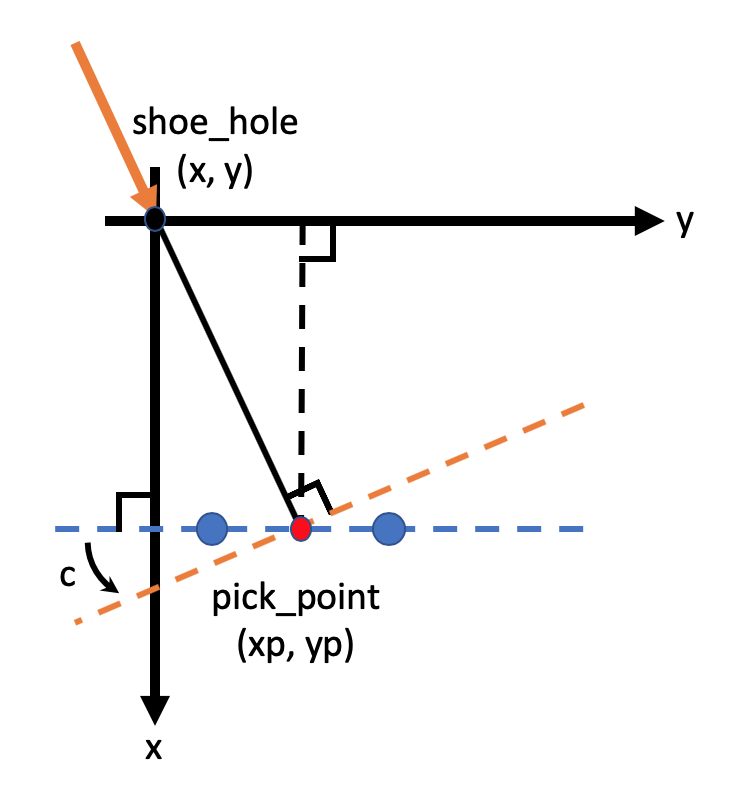
\includegraphics[width = 0.5\columnwidth]{Implementation/mp/lacegrab.png}
\caption{2D Top view that contains the shoe hole position, ideal shoelace pickup position, etc. for top-left case}
\label{lacegrab}
\end{figure}

For this example, the orientation of the shoelace is considered to be aligned with this direction. Therefore, when YuMi's gripper is perpendicular to it, YuMi will have the highest probability to complete this task. In other words, the two fingers of the gripper should be at the two orange points respectively, which aligns with orange dash line. In this case, when the gripper closes, the shoelace can be grabbed. 

The parameter that controls the rotation on the z-axis is yaw rotation. When YuMi's fingers are at two blue points in Figure \ref{lacegrab}, the yaw rotation is $\frac{\pi}{2}$. Thus, there is an angle $c$ needs to be added, which can be calculated according to Equation \ref{yawcalculation}.

\begin{equation}
c = \arctan \frac{yp - y}{xp - x}
\label{yawcalculation}
\end{equation}

Considering both top-left and top-right cases, the available range of $c$ is $[-\frac{\pi}{2}, \frac{\pi}{2}]$. When this condition is satisfied, the final grabbing pose can be written as Equation \ref{grabpose}. The pre-grabbing pose is same as the grabbing pose except its $z$ value is a little bit higher, which allows !!!!!!!!!!

\begin{equation}
Grabbing\_pose = [xp + x\_offset, yp + y\_offset, zp + z\_error, 0, \pi, c + \frac{\pi}{2} - 0.26]
\label{grabpose}
\end{equation}

Notice that, here, the offset for 3D location is different form that of $Prepur\_pose$ and $Insertion\_pose$. This is because this time the gripper does not perform any roll and pitch rotations from its default orientation. In addition, $-0.26$ is added to yaw rotation by taking into account of the !!!!!!!!!!!!!!!!

\begin{figure}[H]
\centering

\includegraphics[width = 0.3\columnwidth]{images/ph.png}
\caption{0.26}
\label{0.26}
\end{figure}

\begin{figure}[H]
\centering
\subfigure[]{
\includegraphics[width = 0.19\columnwidth]{images/ph.png}}
\subfigure[]{
\includegraphics[width = 0.19\columnwidth]{images/ph.png}}
\subfigure[]{
\includegraphics[width = 0.19\columnwidth]{images/ph.png}}
\subfigure[]{
\includegraphics[width = 0.19\columnwidth]{images/ph.png}}
\subfigure[]{
\includegraphics[width = 0.19\columnwidth]{images/ph.png}}
\caption{Example of pulling shoelace out}
\end{figure}